\section{Using \padx{} to Query Ad Hoc Data}
\label{section:padx}

\begin{figure}
\begin{center}
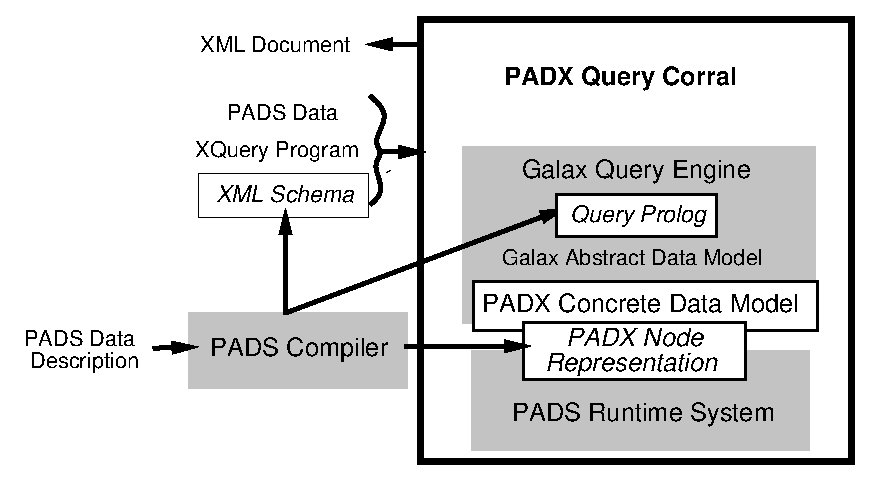
\epsfig{file=padx-arch.ps,width=0.47\textwidth}
\end{center}
\caption{\padx{} Architecture}
\label{figure:padx-arch}
\end{figure}

Figure~\ref{figure:padx-arch} depicts the \padx{} architecture.  From
a \pads{} description, the compiler generates an XML Schema
description that specifies the virtual XML view of the corresponding
\pads{} data; an XQuery prolog that imports the corresponding schema
and that associates the input data with the correct schema type; and a
type-specific library that maintains the information necessary to
support the \padx{} data model.

An instance of the \padx{} runtime system, called the ``query
corral'', consists of the \Galax{} query engine, a type-specific query
prolog, the \padx{} implementation of the \Galax{} data model, a
type-specific \padx{} library, and the \pads{} runtime system.  Note
that the resulting query corral is \emph{specialized} for a particular
\pads{} description.  From the query prolog, it imports the XML Schema
that corresponds to the underlying type-specific library, i.e., it
does permit the query writer to import an arbitrary schema.  This
restriction guarantees that the XQuery program is typed with respect
to the correct XML Schema and that the underlying data model is an
instance of the specified XML Schema.  At runtime, the query corral
takes an XQuery program and a \pads{} data source and produces the
query result in XML.  We discuss the problem of producing native
\pads{} values in Section~\ref{section:future}. 

Section~\ref{section:pads} describes the output of the \pads{}
compiler.  Here, we focus on the mapping from a description to XML
Schema and on the features of the type-specific data model.

\subsection{Virtual XML view of PADS data}

The fragment of the XML Schema in Figure~\ref{figure:dibbler-schema}
corresponds to the description in Figure~\ref{figure:dibbler}.  We use
this example to illustrate the mapping of a \pads{} description to XML
Schema.

Each compound type is mapped to a complex schema type with a
particular content model.  A \kw{Pstruct} is mapped to a complex type
that contains a sequence of local elements, each of which corresponds
to one field in the \kw{Pstruct}.  For example, the \kw{Pstruct}
\cd{order\_header\_t} is mapped to the complex type
\cd{order\_header\_t}, which contains an element declaration for the
field \cd{order\_num}, among others.  Each complex type also includes
an optional \cd{pd} element that corresponds to the type's parse
descriptor.  The \cd{pd} element is absent if no errors occurred
during parsing, but if present, permits an analyst to easily identify
the kind and location of errors in the source data.  For example, this
expression returns the locations of all orders that contain
at least one error: \cd{$pads/Psource/orders/elt/pd/loc}. 

\cut{``Error-aware'' mapping from PADS type system to isomorphic XML}
Schema. 

The XML Schema types for other compound types annotated
with corresponding fields from PADS rep, e.g., arrays have a length. 


Extra level of indirection in representation of arrays---wrap each
item in an element. 

A \kw{Punion} is mapped to a choice of elements, each of which
corresponding to one field in the \kw{Punion}. 


\begin{figure*}
\begin{small}
\begin{code}
<xs:schema targetNamespace="\kw{file:/example/sirius.p}"
           xmlns="file:/example/sirius.p"
           xmlns:xs="http://www.w3.org/2001/XMLSchema"
           xmlns:p="http://www.padsproj.org/pads.xsd">
<xs:import namespace = "http://www.padsproj.org/pads.xsd".../>
...
<xs:complexType name="\kw{order_header_t}">
 <xs:sequence>
  <xs:element name="\kw{order_num}"     type="\kw{p:val_Puint32}"/>
  <xs:element name="\kw{att_order_num}" type="\kw{p:val_Puint32}"/>
  <xs:element name="\kw{ord_version}"   type="\kw{p:val_Puint32}"/>
  <!-- More local element declarations -->
  <xs:element name="\kw{pd}"            type="\kw{p:PStruct_pd}" minOccurs="0"/>
 </xs:sequence>
</xs:complexType>
<!-- More complex type declarations -->
<xs:complexType name="\kw{orders_t}">
 <xs:sequence>
  <xs:element name="\kw{elt}"    type="\kw{order_t}" maxOccurs="unbounded"/>
  <xs:element name="\kw{length}" type="\kw{p:Puint32}"/>
  <xs:element name="\kw{pd}"     type="\kw{p:Parray_pd}" minOccurs="0"/>
 </xs:sequence>
</xs:complexType>
...
<xs:element name="PSource" type="summary"/>
</xs:schema>
\end{code}
\end{small}
\caption{Fragment of XML Schema for \dibbler{} \pads{} description.}
\label{figure:dibbler-schema}
\end{figure*}

Each base type is mapped to an XML Schema simple type.  Since the base
types do not change, the corresponding XML Schema types are defined
once in \cd{pads.xsd}, which is imported into all generated schemata. 
\begin{small}
\begin{code}
<xs:simpleType name="Puint32">
  <xs:restriction base="xs:unsignedInt"/>
</xs:simpleType>
<xs:complexType name="\kw{val_Puint32}">
  <xs:\kw{choice}>
   <xs:element name="\kw{val}" type="\kw{p:Puint32}"/>
   <xs:element name="\kw{pd}"  type="\kw{p:Pbase_pd}"/>
  </xs:\kw{choice}>
</xs:complexType>
<xs:complexType name="\kw{Pbase_pd}">
 <xs:sequence>
   <xs:element name="\kw{pstate}"  type="\kw{p:Pflags_t}"/>
   <xs:element name="\kw{errCode}" type="\kw{p:PerrCode_t}"/>
   <xs:element name="\kw{loc}"     type="\kw{p:Ploc_t}"/>
 </xs:sequence>
</xs:complexType>
\end{code}
\end{small}



Extra level of indirection for base types: must contain the value of
the base type and an optional parse-descriptor, if an error has
occurred. 

We don't take complete advantage of XML Schema, e.g., Penum types
could be modeled by XML Schema enumeration simple types, but currently
unsupported.

Example of query prolog. 
\begin{figure*}
\begin{small}
\begin{code}
import schema default element namespace "\kw{file:/example/sirius.p}";
declare variable \kw{$pads} as \kw{document-node(PSource)} external; 
\end{code}
\end{small}
\caption{\padx{} generated query prolog}
\label{figure:padx-query-prolog}
\end{figure*}

How to access data files:  fn:doc("pads:/example/sirius.data");

\subsection{Physical Data Model}

% Part of PADX implementation are generic functions that implement data
% model accessors.  PADS compiler generates type-specific functions for
% walking virtual XML tree.  Relate back to type-specific library
% functions mentioned in last section.

% Implementation of Galax's Abstract Tree Model.

% Minimum necessary to implement Galax DM:

% 1. Generic implementations of the DM accessors: axis::node-test(), children(),
%    attributes(), name(), etc. 

% 2. On PADX-side, we have a virtual handle for each node in the XML
%    tree--we call that a node rep.  Node rep contains pads handle
%    (maintains state for PADS parser); type-specific vtable of DM
%    accessors; other stuff...

%    Give example of vtable for event\_t and possibly code for
%    kthChildByName. 

In order to export \pads data as XML, we wrap data in {\em node}
datastructures containing all the information relevant to XML. Handles
to these nodes are then passed to \galax which can invoke very simple
queries on the node, such as ``what is your name? give me a list of
your children, etc.''  Within \galax, the interface with pads is
wrapped in a module that exports the \galax Data Model interface to
the \galax query engine.

The physical data model provides the means to query \pads data by
walking a virtual XML tree.  At the core of the physical data model
are the \cd{node} data structure and the generic node interface.
Together, these play the same role as an abstract class in C++ and
Java. They specify only common fields used by all nodes, and the
required accessor methods. They do not, however, provide any method
implementations. They are fixed elements of the system, independant of
any particular \pads{} types.

\begin{figure*}
{\small
\begin{verbatim}
nodeRep      PADX_generic_parent      (nodeRep n)

const char*  PADX_generic_name        (nodeRep n)
const char*  PADX_generic_kind        (nodeRep n)
item         PADX_generic_typed_value (nodeRep n)
const char*  PADX_generic_string_value(nodeRep n)

nodeRep      PADX_generic_kth_child         (nodeRep n, childIndex idx)
nodeRep      PADX_generic_kth_child_named   (nodeRep n, childIndex idx, 
                                             const char *name)
\end{verbatim}
}
\caption{The generic node interface}
\label{fig:generic-node-interface}
\end{figure*}

The generic node interface defines the functions that are available to the
\pads{} data model implementation for use on nodes. The relevant portions of
this interface are shown in \figref{fig:generic-node-interface}.

The {\tt kth-child} function returns the kth child of the node
starting from zero. The {\tt kth-child-named} function returns the node's kth
child with the specified name. This function is most relevant to
arrays, where all of the elements are given the same name ``elt.''
For both functions, {\tt NULL} is a valid result, indicating that the
requested child does not exist.

\begin{figure}
{\small
\begin{verbatim}
struct PDCI_node_s {
  const char              *name;
  const char              *kind;
  PDCI_node_t             *parent;

  void                    *m;
  void                    *pd;
  void                    *rep;

  const PDCI_vtable_t     *vt;
  P_t                     *pads;
  ...
}
\end{verbatim}
}
\caption{The node structure}
\label{fig:node-struct}
\end{figure}

The basic contents of the \cd{node} data structure are shown in
\figref{fig:node-struct}. All nodes have a name and a kind, stored as
C-strings. Additionally, all nodes but the document node have a parent
in the document, hence the parent field that points to another node.
Next we have the mask, representation and parse-descriptor fields. As
these elements of the node are type-specific, they are all typed as
\vptr.

Next we have the pointer to the node's virtual table, {\tt vt}. The
virtual functions will often need a valid \pads handle to execute
correctly. Therefore, we also include a pads handle field in each
node.

\subsubsection{Node implementations}
The PADS compiler generates the type-specific implementations of the
node functions, along with the other type-specific tools.  The
type-specific knowledge available at compile time is used not only to
manipulate the node's data appropriately but also to select the (type)
correct implementations of children nodes, when necessary.  For
example, for structures, the children are the parse-descriptor and the
fields of the structure, each with their own type and corresponding
node implementation.  For arrays, the children are the
parse-descriptor, the array length, and a list of nodes with name
``elt,'' corresponding to the elements of the array. The
parse-descriptor is accessed through an implementation for array pds,
the length field through an implementation for 32-bit integers, and
each of the elements with the implementation appropriate to the
particular element type of the array. Other datatypes are analagous.

It is important to note that the XML representations of \pads data
integrate each datastructure's parse-descriptor with the data,
exporting it as a child of the datastructure itself. This design
allows queries to select (or ignore) nodes based on the contents of
their parse-descriptors in an easy and efficient manner. It also means
that their are a fixed number of pd node implementations (approx. one for
each type constructor), as opposed to the unlimited number of data
node implementations, generated fresh for each new \pads{} type.

In order to support the full range of \pads datatypes,
the node data structure is designed using ``{\tt void *}
polymorphism.'' That is, anywhere that the node architecture is not
specific to a particular type, we use a {\tt void *} type. In this
way, we can write type-neutral code to manipulate data nodes. For
example, the rep and pd pointers in each node are typed as {\tt void
  *}. 

Each type-specific implementation will (down)cast such pointers to the
appropriate type before use, relying on the (assumed) invariant that
no only code specific to that type has manipulated those pointers.

\subsubsection{Data input strategies: when to actually read from PADS data?}

The flexibility of the node interface goes beyond support for
arbitrary \pads{} types. It also allows us, for each type, to support
alternative implementations of the interface. We take advantage of
this flexibility to support multiple data input strategies: bulk-read
and two forms of on-demand read.

\begin{enumerate}
\item Bulk read: Materialize entire PADS representation, populate all of the PADS
reps.  Then PADX DM lazily invoked the DM accessors over this data.
Problem: if data is big, it's all sitting in memory, even if the query
only touches a fragment of the virtual XML tree.

\item On-demand, sequential read: same as smart but does not preserve meta-data.
   Does not permit multiple scans of data source. 

\item On-demand, random access read: 
Many common queries permit sequential, streamed access to underlying
XML source.  Give an example.  

Smart node rep, preserves meta-data about previously read records, but
re-uses memory for reading next item.  This rep permits multiple scans
of input (semantic problem is that DM must preserve node identity),
but slowly. 

Heuristic: records are a good level of granularity to read.   Each
smart node corresponds to one record.  When next smart node is
accessed, a little meta-data is preserved: the node rep and the
records location in the file (so we can re-read it if necessary).
\end{enumerate}

Put in PADX signatures for constructing a new node and accessing
kthChild. 

Something about query evaluation:
Although we have not explored custom evaluation plans 
Galax's algebra or optimizer are particularly interesting in the 
\padx{}, we expect to do so 

%%% Local Variables: 
%%% mode: latex
%%% TeX-master: "paper"
%%% End: 
